%\vspace{-2pt}
\section{Graph-based Try-Catch Necessity Checking Model}
\label{detect:sec}

\begin{figure}[t]
	\centering
	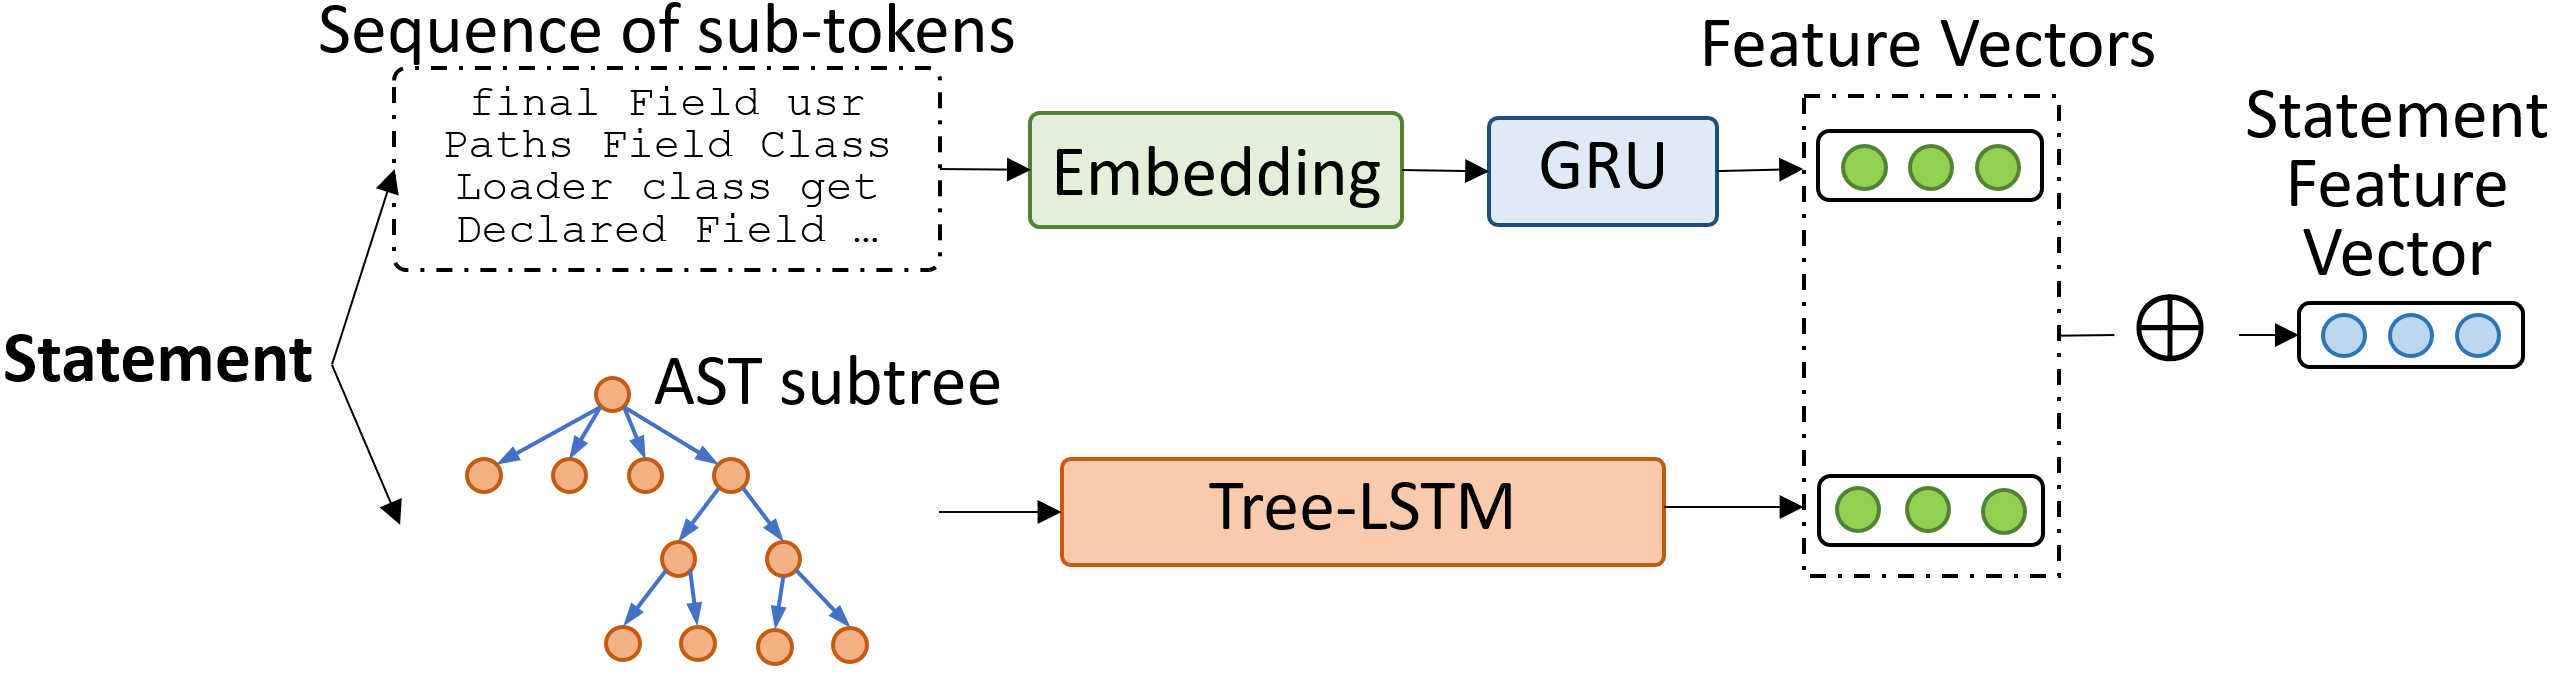
\includegraphics[width=3.2in]{features.png}
        \vspace{-0.08in}
	\caption{Code Representation Learning for Statement}
%        \vspace{-0.05in}
	\label{fig:feature}	
\end{figure}

%Tien
This section describes our graph-based {\xblock} model. We first
explain how we build the context-aware representation learning for the
given code, and then how we use such learned vectors for the detection
of the presence of \code{try-catch} block using R-GCN~\cite{yi}.

\subsection{Code Representation Learning}
\label{replearn:sec}

Let us present how we build the vectors for code
features. We aim to capture the lexical and structural features for a
statement, while the PDG captures the dependencies among statements.

\vspace{-1pt}
\subsubsection{Sequence of Sub-tokens of a Statement}

At the lexical level, the lexical content of a statement is
represented via a sequence of the sub-tokens. The sub-token
granularity has been shown to have higher regularity than the
tokens~\cite{icse20-methodname}. Each statement is tokenized using
CamelCase or Hungarian convention. Then, only variables, methods,
fields, and class' names are kept. The sub-tokens with one character
are removed to avoid noises. As an example, in
Figure~\ref{fig:example1} at line 2, we collect the sequence of
sub-tokens as follows: \code{final}, \code{Field}, \code{usr},
\code{Paths}, etc. Then, we use a word embedding~\cite{glove2014} to
build the vectors for the sub-tokens, together with Gate Recurrent
Unit (GRU)~\cite{chung2014empirical} to build the feature vector for
the sequence of sub-tokens for the current statement.

%At the lexical level, we capture the content of a statement in term of
%the sequence of sub-tokens. We choose the sub-token granularity
%because the sub-tokens are more likely to be repeated than the entire
%lexical tokens in source code~\cite{icse20-methodname}.
%We tokenize each statement and keep only the variables, method and
%class names. The names are broken into sub-tokens using CamelCase or
%Hungarian convention. We remove the sub-tokens with one character to
%avoid the influence of noises. For example, in
%Figure~\ref{fig:feature}, the tokens of $S_{27}$ are collected and
%broken down into the sequence: \code{copy}, \code{to}, \code{user},
%\code{arg}, {\em etc}. Then, we use GloVe~\cite{glove2014}, to build the
%vectors for tokens, together with Gate Recurrent Unit
%(GRU)~\cite{chung2014empirical} to build the feature vector for the
%sequence of sub-tokens for $S_{27}$.
%GloVe is known to capture well semantic similarity among tokens. GRU
%is chosen to summarize the sequence of vectors into one feature vector
%for the next step.

%In the case of a vulnerable statement and its fixed ones, we combine
%them via multiplication to get the feature vector.

%is an effective method for measuring the linguistic or semantic
%similarity of the tokens. We need the GRU to summarize the sequence of
%vectors into one feature vector for the next step.

%{\tool} use GloVe here because we would like to use a word
%representation tool to transform the natural language tokens into
%vectors which could be used in GCN model. After apply GloVe, the
%sequence of tokens will be transformed into a sequence of vectors. In
%order to get only one vector for one feature, we use GRU here to
%summarize the sequence of vectors into one feature vector for the next
%step.

%{\tool} braking the statement $v$ into sequence and using a GRU model \cite{} to summarize the sequence as the second feature representation vector $F_{v,2}$ for statement $v$ by only taking variable, method, and class names and using the CamelCase and Hungarian convention to break each name into a sequence of sub-tokens and in order to avoid influence of basis, {\tool} removed one character length sub-tokens.

%\subsubsection{{\bf Code structure of the statement}}
%\label{ast:sec}

%Tien
%\vspace{0.06in}
%\noindent {\bf 2. Code Structure of a Statement.}

\vspace{-1pt}
\subsubsection{Code Structure of a Statement}

At the syntactic level, we aim to capture the code structure via the
AST. In Figure~\ref{fig:feature}, we parse the code and extract the
AST subtree for the given statement, and then feed it to the Tree-LSTM
model~\cite{tai2015improved}, which produces a feature vector to
capture the structure.

%Tree-based LSTM model is known for capturing well tree structures.

%\vspace{-1pt}
%\subsubsection{Variables and Types}

%For each node ({\em i.e.}, a statement), we collect the names of the
%variables and their static types at their locations, break them into
%the sub-tokens. For example, we collect the variable \code{s$\_$cmd}
%and its static type \code{cross$\_$ec$\_$command}.
%We use the same vector building techniques as for the sub-token
%sequences as in the feature~1, including GloVe and GRU, to apply on the
%sequences of the sub-tokens built from the variables' names ({\em e.g.},
%\code{s$\_$cmd}) and those from the variables' types ({\em e.g.},
%\code{cross$\_$ec$\_$command}).

%\vspace{-1pt}
%\subsubsection{Surrounding Contexts}

%During training, for a statement $s$, we also encode the statements
%surrounding $s$, which we refer to as {\em context}.  We have two
%contexts. Data- and control-dependency contexts contain the
%statements having such dependencies with the current statement.
%For example, the data-dependency context for $S_{27}$ includes
%the statements at the lines 31, 22, 13, 10, and 6.  If the control
%dependencies are considered, the statements with control dependencies
%with $S_{27}$ at the lines 29, 25, 23, and 13 are included.
%
%The vectors for the statements in the context are calculated via GloVe
%and GRU as described earlier. Because the number of dependencies could be
%different, the lengths of the GRU model inputs could be
%different. Thus, we apply zero padding with a masking layer, allowing the model to skip the zeros at the end of the sequence of
%sub-tokens. Those zeros will not be included in training.

%\vspace{-1pt}
%\subsubsection{Attention-Based Bidirectional GRU} 

%After having all vectors for the features $F_1$, $F_2$, ..., we use a
%bi-directional GRU and an attention layer to learn the weight
%vector $W_i$ for each feature $F_i$, based on the hidden states from
%that model.  Then, we compute the weighted vector for each feature by
%multiplying the original vector for the feature by the weight, that is, we have $F'_i$ = $W_i$.$F_i$.

%Finally, we need to consider the impacts from the {\em dependent statements to the current statement in the PDG}. The rationale is that those
%neighboring statements in the PDG must have the influence on the
%current statement if one of them is vulnerable. For example, the
%neighboring statements for $S_{27}$ in the PDG include the statements
%at lines 6, 22, 25, and 29. Thus, we combine and summarize them into
%the final feature vector $F_{S27}$ for the statement $S_{27}$
%as follows:
%\begin{equation}\label{eq:9}
%F_{S27} = \sum_i{W_i{Concat(h(F'_i,j))}}
%\end{equation}
%$W_i$ is the trainable weight for combination; $Concat$ is the
%concatenate layer to link all values into one vector; $h$ is the
%hidden layer to summarize vector into a value; $i$ = S6, S22, S25,
%S27, S29; $j$ is feature index. $F_{27}$ is used in the next step
%with GCN model for detection.

\subsection{\code{Try-catch} Block Checker with R-GCN}
\label{model:sec}

\begin{figure}[t]
	\centering
	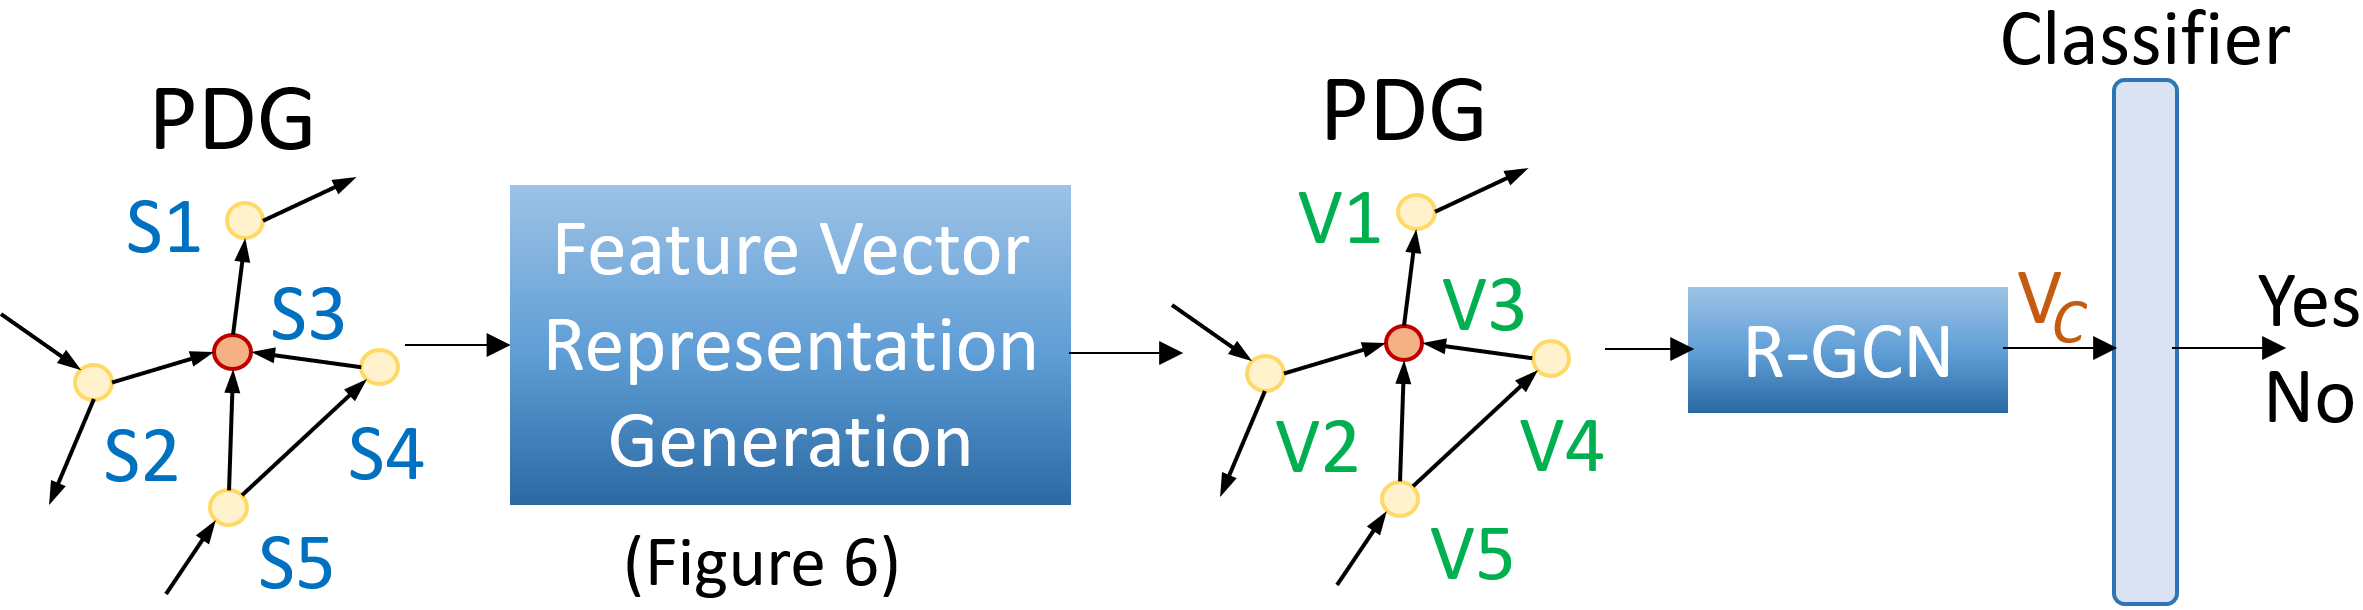
\includegraphics[width=3.4in]{xblock.png}
  %      \vspace{-0.1in}
	\caption{\code{Try-catch} Block Checker with R-GCN}
	\label{fig:gcn}	
\end{figure}

Figure~\ref{fig:gcn} presents how we use Feature-Attention GCN model
(FA-GCN)~\cite{FAGCN} for detection. The rationale is that FA-GCN can
deal well with the graphs with sparse features (not all the statements
share the same properties), and potentially noisy features in a PDG.
%Figure~\ref{fig:gcn} explains how {\tool} detects vulnerable code using
%FA-GCN.
First, we parse the method $M$ into PDG. Similar to CNN using the
filter on an image, FA-GCN performs sliding a small window along all
the nodes (statements) of the PDG. For example, in
Figure~\ref{fig:gcn}, the window marked with A for the node
$S27$ consists of itself and the neighboring statements/nodes $S6$,
$S22$, $S25$, and $S29$. Another window (marked with B) is
for the node $S23$, including itself and the neighboring nodes:
$S22$ and $S25$. For each window, FA-GCN generates the feature
representation matrix for the statement at the center. For example,
for the window centered at $S27$, it generates the feature vector
$F_{S27}$ for $S27$, using the process explained in
Figure~\ref{fig:feature}. From the representation vectors for
all statements, FA-GCN uses a join layer to link all these vectors
into the Feature Matrix $\mathcal{F}_{m}$ for method $M$. A row in
$\mathcal{F}_m$ corresponds to a window in~PDG.

Next, FA-GCN performs the convolution operation by first calculating
the symmetric normalized Laplacian matrix~$\tilde{A}$~\cite{GCN16},
and then calculating the convolution to generate the representation
matrix $M_{m}$ for the method $m$. After that, we use the traditional
steps as in a CNN model: using a spatial pyramid pooling layer (to
normalize the method representation matrix into a uniform size, and
reduce its total size), and connecting its output to a fully connected
layer to transform the matrix into a vector $V_m$ to represent
$m$. With $V_m$, we perform classification by using two hidden layers
(controlling the length of vectors and output) and a softmax function
to produce a prediction score for $m$. We use those scores as {\em
  vulnerability scores to rank the methods} in a project. The decision
for $m$ as $\mathcal{V}$ or $\mathcal{NV}$ is done via a trainable
threshold on the prediction score~\cite{li2018vuldeepecker,li2019improving}.

%The model also assigns a score for $m$. We consider those scores



%--- old ----
%Next, FA-GCN performs the convolution operation by first
%calculating the symmetric normalized Laplacian matrix~$\tilde{A}$:
%\begin{equation}\label{eq:7}
%\tilde {A} =D^{-\frac{1}{2}}(I+A)D^{-\frac{1}{2}}
%\end{equation}
%Where $D$ is the degree matrix, $I$ is the identity matrix, and $A$ is
%the adjacency matrix. With the symmetric normalized Laplacian matrix,
%FA-GCN performs the convolution calculation to generate the
%representation matrix $M_{m}$ for method $M$:
%\begin{equation}\label{eq:8}
%{M}_{m}  = g(\tilde{A}\mathcal{F}_mW)
%\end{equation}
%Where $W$ is the weight matrix, and $g$ is an activation function.

%Next, we perform the classification of $\mathcal{V}$ or $\mathcal{NV}$
%for the given method $M$. To achieve that, we use a spatial pyramid
%pooling layer (with the same role as in the CNN model) to normalize
%the method representation matrix, into a uniform size, and then reduce
%the total size of that matrix. Then, we send the output from the
%pooling layer into a fully connected layer to transform the matrix
%into a vector to represent the method $m$. Let us call it the
%representation vector for $V_{m}$.
%
%After having the vector $V_{m}$ for $M$, {\tool} uses a classifier for
%prediction. The classifier is built by two hidden layers, which are
%used to control the length of vectors and output, and the Softmax
%activation function. We use this classifier since it is simple and
%common used in many classification problem~\cite{li2018vuldeepecker,
%  li2019improving}.
%----



%These pooling and fully connected layers are widely used in the CNN
%model, and they play the same role in the FA-GCN model.

%%%%%%%%%%%%%%%%%%%%%%%%
%The
%statement representation matrix for $S27$ is also marked with (A),
%corresponding to the window (A) in the PDG. Similarly, the matrix for
%$S23$ is marked with (B) for the window (B) in the PDG.
%%%%%%%%%%%%%%%%%%%%%%%%
%After we talked about the details about the feature representation generation. We would like to introduce the process for {\tool} to use it to do the vulnerability detection. As we mentioned, first of all, we build the program dependency graph (PDG) for the incoming method $M$. Then, to do the convolution calculation, {\tool} swipes on the PDG for each node just like the CNN \cite{} model swipe the filters on the images. For example, in figure \ref{fig:gcn}, you can see that the blue window and green window on the PDG shows two swipes. The green window shows that the {\tool} is swiping on the \textit{S27} and also including the neighborhood statements include \textit{S6, S22, S25, S29}. Also, the same as the green window, the blue window shows that the {\tool} is swiping on node \textit{S23} with neighborhood statements \textit{S22, S25}.
%After having each statement swiping, we use them to generate the statement representation vectors. We use \textit{S27} as an example. After having the green window, {\tool} firstly do the feature representation generation which is shown in figure \ref{fig:feature} to generate the feature matrix $M_{S27}$ for \textit{S27}. Then we calculate the symmetric normalized Laplacian matrix $\tilde {A}$ by:
%\begin{equation}\label{eq:7}
%\tilde {A} =D^{-\frac{1}{2}}(I+A)D^{-\frac{1}{2}}
%\end{equation}
%%%%%%%%%%%%%%%%%%%%%%%%
%After this step, for each statement/node, we have a statement
%representation matrix (e.g., $M_{S27}$).
%%%%%%%%%%%%%%%%%%%%%%%%



%%%%%%%%%%%%%%%%%%%%
%To achieve that, we need to combine the representations for all
%the statements. We use a spatial pyramid pooling layer to
%normalize the statement representation matrix, e.g., $M_{S27}$ into a
%uniform size, and then reduce the total size of that matrix. Then, we
%send the output from the pooling layer into a fully connected layer to
%transform the matrix into a vector to represent the statement $S27$.
%Let us call it the statement representation vector for $V_{S27}$.
%These pooling and fully connected layers are widely used in the CNN
%model, and they play the same role in the FA-GCN model.
%%%%%%%%%%%%%%%%%%%%
%Because {\tool} needs to do the classification on the whole method which requires to combine all statement representation information together, for each statement, such as \textit{S27}, {\tool} firstly uses a spatial pyramid pooling layer to normalize the $M_{S27, cov}$ into a uniform size and then reduce the total size of the matrix. Then, {\tool} send the output from spatial pyramid pooling layer into a fully connected layer to transform the matrix into statement representation vector for \textit{S27}. These pooling and fully connected layers are also been widely used in CNN model and they playing the similar roles in CNN model.




%%%%%%%%%%%%%%%%%%%%
%After having all statement representation vectors, {\tool} use a join
%layer to link these vectors together and then use the resulting vector
%as the method representation vector for the entire method $M$. Next,
%{\tool} uses a classifier for prediction. The classifier in {\tool} is
%built by 2 hidden layers which are used to control the length of
%vectors and output, and apply the Softmax activation function for
%classification. We use this classifier because it is simple and common
%used in many DL-based classification problem \cite{yi}.
%%%%%%%%%%%%%%%%%%%
%After having the feature-attention based representation vector $x_{V,atte}$, {\tool} generates summarized $N \times D$ feature matrix $X_M$ where $N$ is number of nodes and $D$ is the number of node features. With this matrix, {\tool} is able to preserve the first-order neighborhood relations between statement, and the relationship feature matrix $\tilde{X_M}$ could be computed by:

%\begin{equation}\label{eq:7}
%\tilde {X_M}  = g(\tilde{A}X_MW)
%\end{equation}

%Where $\tilde {A} =D^{-\frac{1}{2}}(I+A)D^{-\frac{1}{2}}$ is the normalized symmetric adjacency matrix, $W$ is the weight matrix, and $g$ is an activation function ReLU represented by $g= max(0, x)$.

%After having $\tilde X_M$, {\tool} is able to use a convolutional layer to classify the whole graph into two groups including \textit{vulnerable} and \textit{non-vulnerable} which is the output of this step in {\tool}.
